\section{Getting Started}

This Getting Started guide is written with a default installation in mind, meaning that some parts may not apply if a custom installation was used.
When the \textit{allpix} binary is used, this refers to the executable installed in \text{bin/allpix} in your installation path.
Remember that before running any \apsq simulation, ROOT and likely Geant4 should be initialized.
Refer to Section~\ref{sec:initialize_dependencies} on instructions how to load these libraries.

\subsection{Configuration Files}
\label{sec:configuration_files}
The framework is configured with simple human-readable configuration files.
The configuration format is described in detail in Section~\ref{sec:config_file_format}.
The configuration consists of several section headers within $[$ and $]$ brackets and a section without header at the start.
Every section contain a set of key/value pairs separated by the \texttt{=} character.
Comments are indicated using the has symbol (\texttt{\#}).

The framework has the following three required layers of configuration files:
\begin{itemize}
\item The \textbf{main} configuration: The most important configuration file and the file that is passed directly to the binary.
Contains both the global framework configuration and the list of modules to instantiate together with their configuration.
An example can be found in the repository at \textit{etc/example.conf}.
More details and a more thorough example are found in Section~\ref{sec:main_config}.
\item The \textbf{detector} configuration passed to the framework to determine the geometry.
Describes the detector setup, containing the position, orientation and model type of all detectors.
An example is available in the repository at \textit{etc/example\_detector.conf}.
Introduced in Section~\ref{sec:detector_config}.
\item The detector \textbf{models} configuration.
Contain the parameters describing a particular type of detector.
Several models are already provided by the framework, but new types of detectors can easily be added.
See \textit{models/test.conf} in the repository for an example.
Please refer to Section~\ref{sec:adding_detector_model} for more details about adding new models.
\end{itemize}

In the following paragraphs, the available types and the unit system are explained and an introduction to the different configuration files is given.

\subsubsection{Parsing types and units}
\label{sec:config_values}
The \apsq framework supports the use of a variety of types for all configuration values.
The module specifies how the value type should be interpreted.
An error will be raised if either the key is not specified in the configuration file, the conversion to the desired type is not possible, or if the given value is outside the domain of possible options.
Please refer to the module documentation in Section~\ref{sec:modules} for the list of module parameters and their types.
Parsing the value roughly follows common-sense (more details can be found in Section~\ref{sec:accessing_parameters}).
A few special rules do apply:
\begin{itemize}
\item If the value is a \textbf{string}, it may be enclosed by a single pair of double quotation marks (\texttt{"}), which are stripped before passing the value to the modules.
If the string is not enclosed by quotation marks, all whitespace before and after the value is erased.
If the value is an array of strings, the value is split at every whitespace or comma (\texttt{'}) that is not enclosed in quotation marks.
\item If the value is a \textbf{boolean}, either numerical (\texttt{0}, \texttt{1}) or textual (\texttt{false}, \texttt{true}) representations are accepted.
\item If the value is a \textbf{relative path}, that path will be made absolute by adding the absolute path of the directory that contains the configuration file where the key is defined.
\item If the value is an \textbf{arithmetic} type, it may have a suffix indicating the unit.
The list of base units is shown in Table~\ref{tab:units}.
\end{itemize}

\begin{warning}
  If no units are specified, values will always be interpreted in the base units of the framework.
  In some cases this can lead to unexpected results.
  E.g. specifying a bias voltage as \texttt{bias\_voltage = 50} results in an applied voltage of \SI{50}{\mega\volt}.
  Therefore it is \textbf{strongly recommended} to always specify units in the configuration files.
\end{warning}

The internal base units of the framework are not chosen for user convenience but for maximum precision of the calculations and in order to avoid the necessity of conversions in the code.

\begin{table}[tbp]
\centering
\caption{List of units supported by \apsq}
\label{tab:units}
\begin{tabular}{|l|l|l|}
\hline
\textbf{Quantity}                 & \textbf{Default unit}                   & \textbf{Auxiliary units} \\ \hline
\multirow{6}{*}{\textit{Length}}  & \multirow{6}{*}{mm (millimeter)}        & nm (nanometer)           \\ \cline{3-3}
                                  &                                         & um (micrometer)          \\ \cline{3-3}
                                  &                                         & cm (centimeter)          \\ \cline{3-3}
                                  &                                         & dm (decimeter)           \\ \cline{3-3}
                                  &                                         & m (meter)                \\ \cline{3-3}
                                  &                                         & km (kilometer)           \\ \hline
\multirow{4}{*}{\textit{Time}}    & \multirow{4}{*}{ns (nanosecond)}        & ps (picosecond)          \\ \cline{3-3}
                                  &                                         & us (microsecond)         \\ \cline{3-3}
                                  &                                         & ms (millisecond)         \\ \cline{3-3}
                                  &                                         & s (second)               \\ \hline
\multirow{4}{*}{\textit{Energy}}  & \multirow{4}{*}{MeV (megaelectronvolt)} & eV (electronvolt)        \\ \cline{3-3}
                                  &                                         & keV (kiloelectronvolt)   \\ \cline{3-3}
                                  &                                         & GeV (gigaelectronvolt)   \\ \hline
\textit{Temperature}              & K (kelvin)                              &                          \\ \hline
\textit{Charge}                   & e (elementary charge)                   & C (coulomb)              \\ \hline
\multirow{2}{*}{\textit{Voltage}} & \multirow{2}{*}{MV (megavolt)}          & V (volt)                 \\ \cline{3-3}
                                  &                                         & kV (kilovolt)            \\ \hline
\textit{Angle}                    & rad (radian)                            & deg (degree)             \\ \hline
\end{tabular}
\end{table}

Combinations of base units can be specified by using the multiplication sign \texttt{*} and the division sign \texttt{/} that are parsed in linear order (thus $\frac{V m}{s^2}$ should be specified as $V*m/s/s$).
The framework assumes the default units (as given in Table~\ref{tab:units}) if the unit is not explicitly specified.
It is recommended to always specify the unit explicitly for all parameters that are not dimensionless as well as for angles.

Examples of specifying key/values pairs of various types are given below:
\begin{minted}[frame=single,framesep=3pt,breaklines=true,tabsize=2,linenos]{ini}
# All whitespace at the front and back is removed
first_string =   string_without_quotation
# All whitespace within the quotation marks is preserved
second_string = "  string with quotation marks  "
# Keys are split on whitespace and commas
string_array = "first element" "second element","third element"
# Integer and floats can be specified in standard formats
int_value = 42
float_value = 123.456e9
# Units can be passed to arithmetic type
energy_value = 1.23MeV
time_value = 42ns
# Units are combined in linear order
acceleration_value = 1.0m/s/s
# Thus the quantity below is the same as 1.0deg*kV*K/m/s
random_quantity = 1.0deg*kV/m/s*K
# Relative paths are expanded to absolute
# Path below will be /home/user/test if the config file is in /home/user
output_path = "test"
# Booleans can be represented in numerical or textual style
my_switch = true
my_other_switch = 0
\end{minted}

\subsubsection{Main configuration}
\label{sec:main_config}
The main configuration consists of a set of sections specifying the modules used.
All modules are executed in the \emph{linear} order in which they are defined.
There are a few section names which have a special meaning in the main configuration, namely the following:
\begin{itemize}
\item The \textbf{global} (framework) header sections: These are all zero-length section headers (including the one at the beginning of the file) and all sections marked with the header \texttt{[AllPix]} (case-sensitive).
These are combined and accessed together as the global configuration, which contain all parameters of the framework itself (see Section~\ref{sec:framework_parameters} for details).
All key-value pairs defined in this section are also inherited by all individual configurations as long the key is not defined in the module configuration itself.
\item The \textbf{ignore} header sections: All sections with name \texttt{[Ignore]} are ignored.
Key-value pairs defined in the section as well as the section itself are being discarded by the parser.
These section headers are useful for quickly enabling and disabling individual modules by replaing their actual name by an ignore section header.
\end{itemize}

All other section headers are used to instantiate modules.
Installed modules are loaded automatically.
If problems arise please review the loading rules described in Section~\ref{sec:module_instantiation}.

Modules can be specified multiple times in the configuration files, but it depends on their type and configuration if this allowed.
The type of the module determines how the module is instantiated:
\begin{itemize}
\item If the module is \textbf{unique}, it is instantiated only a single time irrespective of the amount of detectors.
These kind of modules should only appear once in the whole configuration file unless a different inputs and outputs are used as explained in Section~\ref{sec:redirect_module_input_outputs}.
\item If the module is \textbf{detector}-specific, it is instantiated once for every detector it is configured to run on.
By default, an instantiation is created for all detectors defined in the detector configuration file (see Section~\ref{sec:detector_config}, lowest priority) unless one or both of the following parameters are specified:
\begin{itemize}
\item \textbf{name}: An array of detector names the module should be executed for.
Replaces all global and type-specific modules of the same kind (highest priority).
\item \textbf{type}: An array of detector type the module should be executed for.
Instantiated after considering all detectors specified by the name parameter above.
Replaces all global modules of the same kind (medium priority).
\end{itemize}
Within the same module, the order of the individual instances in the configuration file is irrelevant.
\end{itemize}

A valid example configuration using the detector configuration above could be:
\begin{minted}[frame=single,framesep=3pt,breaklines=true,tabsize=2,linenos]{ini}
# Key is part of the empty section and therefore the global configuration
string_value = "example1"
# The location of the detector configuration is a global parameter
detectors_file = "manual_detector.conf"
# The AllPix section is also considered global and merged with the above
[AllPix]
another_random_string = "example2"

# First run a unique module
[MyUniqueModule]
# This module takes no parameters
# [MyUniqueModule] cannot be instantiated another time

# Then run detector modules on different detectors
# First run a module on the detector of type Timepix
[MyDetectorModule]
type = "timepix"
int_value = 1
# Replace the module above for `dut` with a specialized version
#   this does not inherit any parameters from earlier modules
[MyDetectorModule]
name = "dut"
int_value = 2
# Run the module on the remaining unspecified detector (`telescope1`)
[MyDetectorModule]
# int_value is not specified, so it uses the default value
\end{minted}

This configuration can however not be executed in practice because MyUniqueModule and MyDetectorModule do not exist.
In the following paragraphs, a fully functional albeit simple configuration file with valid configuration including a detector configuration is presented.

\subsubsection{Detector configuration}
\label{sec:detector_config}
The detector configuration consist of a set of sections describing the detectors in the setup.
Each section starts with a header describing the name used to identify the detector.
All names have to be unique, thus using the same detector name multiple times is not possible.
Every detector should contain all of the following parameters:
\begin{itemize}
\item A string referring to the \textbf{type} of the detector model.
The model should exist in the search path described in Section~\ref{sec:detector_models}.
\item The 3D \textbf{position} in the world frame in the order x, y, z.
See Section~\ref{sec:models_geometry} for details.
\item The \textbf{orientation} specified as Z-X-Z extrinsic Euler angle.
This means the detector is rotated first around the world's Z-axis, then around the world's X-axis and then again around the global Z-axis.
See Section~\ref{sec:models_geometry} for details.
\end{itemize}
Furthermore it is possible to specialize certain parameters of the detector models, which is explained in more detail in Section~\ref{sec:detector_models}.
This allows to quickly adapt e.g. the sensor thickness of a certain detector without altering the actual detector model file.

\begin{figure}[t]
  \centering
  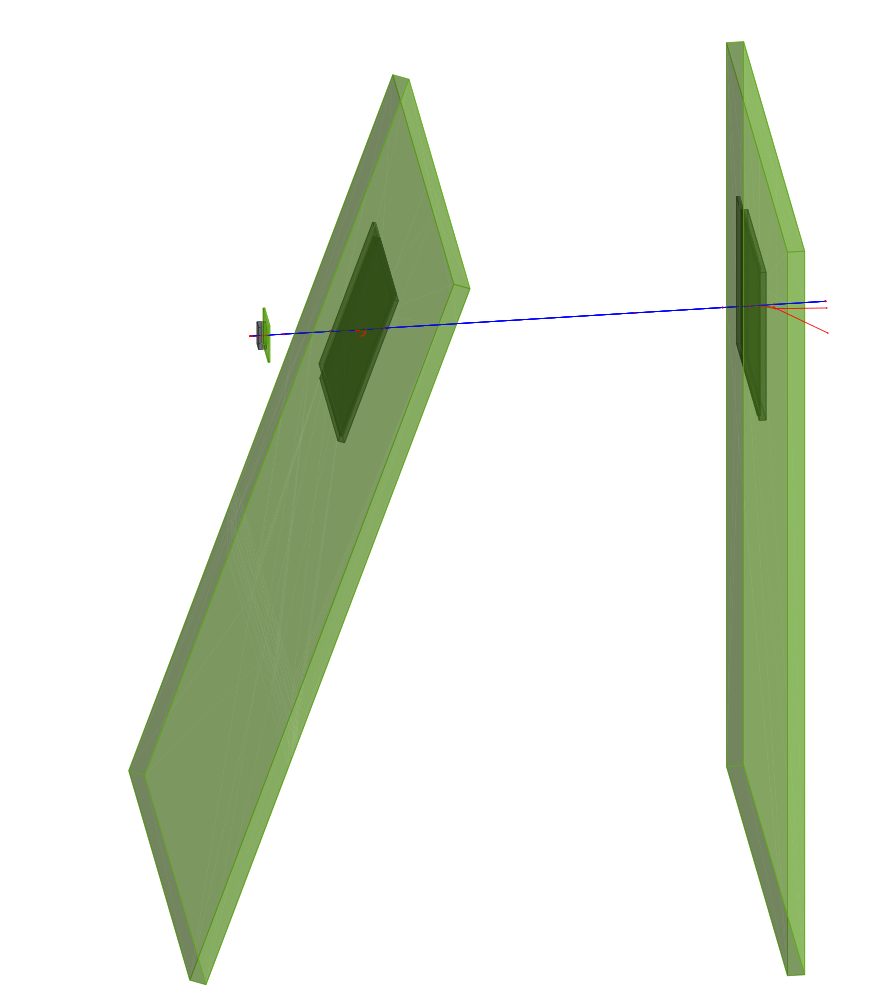
\includegraphics[width=0.6\textwidth]{telescope.png}
  \caption{Visualization of a particle passing through the telescope setup defined in the detector configuration file}
  \label{fig:telescope}
\end{figure}

An example configuration file of one test detector and two Timepix~\cite{timepix} models is:
\inputminted[frame=single,framesep=3pt,breaklines=true,tabsize=2,linenos]{ini}{../../etc/manual_detector.conf}
Figure~\ref{fig:telescope} shows a visualization of the setup described in the file.
This configuration is used in the rest of this chapter for explaining concepts.


\subsection{Framework parameters}
\label{sec:framework_parameters}
The \apsq framework provides a set of global parameters which control and alter its behavior:
\begin{itemize}
\item \textbf{\texttt{detectors\_file}}: Location of the file describing the detector configuration (introduced in Section~\ref{sec:detector_config}).
The only \underline{required} global parameter: the framework will fail if it is not specified.
\item \textbf{\texttt{number\_of\_events}}: Determines the total number of events the framework should simulate.
Equivalent to the amount of times the modules are run.
Defaults to one (simulating a single event).
\item \textbf{\texttt{root\_file}}: Location relative to the \textbf{\texttt{output\_directory}} where the ROOT output data of all modules will be written to.
Default value is \textit{modules.root}.
Directories within the ROOT file will be created automatically for all module instantiations.
\item \textbf{\texttt{log\_level}}: Specifies the lowest log level which should be reported.
Possible values are \texttt{FATAL}, \texttt{STATUS}, \texttt{ERROR}, \texttt{WARNING}, \texttt{INFO} and \texttt{DEBUG}, where all options are case-insensitive.
Defaults to the \texttt{INFO} level.
More details and information about the log levels and how to change them for a particular module can be found in Section~\ref{sec:logging_verbosity}.
Can be overwritten by the \texttt{-v} parameter on the command line.
\item \textbf{\texttt{log\_format}}: Determines the format to display.
Possible options are \texttt{SHORT}, \texttt{DEFAULT} and \texttt{LONG}, where all options are case-insensitive.
More information can be found in Section~\ref{sec:logging_verbosity}.
\item \textbf{\texttt{log\_file}}: File where the log output should be written to in addition to printing to the standard output (usually the terminal).
Only writes to standard output if this option is not provided.
Another (additional) location to write to can be specified on the command line using the \texttt{-l} parameter.
\item \textbf{\texttt{output\_directory}}: Directory to write all output files into.
Subdirectories are created automatically for all module instantiations.
This directory will also contain the \textbf{\texttt{root\_file}} specified via the parameter described above.
Defaults to the current working directory with the subdirectory \textit{output/} attached.
\item \textbf{\texttt{random\_seed}}: Seed for the global random seed generator used to initialize seeds for module instantiations.
A random seed from multiple entropy sources will be generated if the parameter is not specified.
Can be used to reproduce an earlier simulation run.
\item \textbf{\texttt{library\_directories}}: Additional directories to search for module libraries, before searching the default paths.
See Section~\ref{sec:module_instantiation} for details.
\item \textbf{\texttt{model\_path}}: Additional files or directories from which detector models should be read besides the standard search locations.
Refer to Section~\ref{sec:detector_models} for more information.
\end{itemize}

\subsection{Setting up the Simulation Chain}
\label{sec:setting_up_simulation_chain}

In the following, the framework parameters are used to set up a fully functional simulation.
Module parameters are shortly introduced when they are first used.
For more details about these parameters, the respective module documentation in Section~\ref{sec:modules} should be consulted.
A typical simulation in \apsq contains at least the following components.
\begin{itemize}

\item The \textbf{geometry builder}, responsible for creating the external Geant4 geometry from the internal geometry.
In this document, \emph{internal geometry} refers to the detector parameters used by \apsq for coordinate transformations and conversions throughout the simulation, while \emph{external geometry} refers to the constructed Geant4 geometry used for charge carrier deposition (and possibly visualization) only.
\item The \textbf{deposition} module that simulates the particle beam that deposits charge carriers in the detectors using the provided physics list (containing a description of the simulated interactions) and the geometry created above.
\item A \textbf{propagation} module that propagates the charges through the sensor.
\item A \textbf{transfer} module that transfers the charges from the sensor and assigns them to a pixel of the readout electronics.
\item A \textbf{digitizer} module which converts the charges in the pixel to a detector hit, simulating the front-end electronics response.
\item An \textbf{output} module, saving the data of the simulation.
The \apsq standard file format is a ROOT TTree as will be detailed in Section~\ref{sec:storing_output_data}.
\end{itemize}

In this example, charge carriers will be deposited in the three sensors defined in the detector configuration file in Section~\ref{sec:detector_config}.
Only the charge carriers deposited in the sensors of the Timepix detector models are going to be propagated and digitized.
Finally, some detector histograms for the device under test (DUT) will be recorded as ROOT histograms and all simulated objects (including the Monte Carlo truth) are stored to the \apsq ROOT file.
A configuration file implementing this could look like this:
\inputminted[frame=single,framesep=3pt,breaklines=true,tabsize=2,linenos]{ini}{../../etc/manual.conf}

This configuration is available in the repository at \textit{etc/manual.conf}.
The detector configuration file from Section~\ref{sec:detector_config} can be found at \textit{etc/manual\_detector.conf}.

The simulation can be executed by passing the main configuration to the \texttt{allpix} binary as follows:
\begin{verbatim}
$ allpix -c etc/manual.conf
\end{verbatim}
The output should look similar to the sample log provided in Appendix~\ref{sec:example_output}.
The detector histograms such as the hit map are stored in the ROOT file \textit{output/modules.root} in the TDirectory \textit{DetectorHistogrammer/}.

If problems occur when exercising this example, it should be made sure that an up-to-date and properly installed version of \apsq is used (see the installation instructions in Section~\ref{sec:installation}).
If modules and models fail to load, more information about potential issues with the library loading can be found in the detailed framework description in Section~\ref{sec:framework}.

\subsection{Adding More Modules}
In the following, a few basic modules are discussed which might be of use for a very first simulation.

\paragraph{Visualization}
Displaying the geometry and the particle tracks helps both in checking and interpreting the results of a simulation.
Visualization is fully supported through Geant4, supporting all the options provided by Geant4~\cite{geant4vis}.
Using the Qt viewer with the OpenGL driver is the recommended option as long as the installed version of Geant4 is built with Qt support enabled.

To add the visualization, the \texttt{VisualizationGeant4} section should be added at the end of the configuration file.
An example configuration with some useful parameters is given below:
\begin{minted}[frame=single,framesep=3pt,breaklines=true,tabsize=2,linenos]{ini}
[VisualizationGeant4]
# Use the Qt gui
mode = "gui"

# Set transparency of the detector models (in percent)
transparency = 0.4
# Set viewing style (alternative is 'wireframe')
view_style = "surface"

# Color trajectories by charge of the particle
trajectories_color_mode = "charge"
trajectories_color_positive = "blue"
trajectories_color_neutral = "green"
trajectories_color_negative = "red"
\end{minted}
If Qt is not available, a VRML viewer can be used as an alternative, however it is recommended to reinstall Geant4 with the Qt viewer included.
The following steps are necessary in order to use a VRML viewer:
\begin{itemize}
\item A VRML viewer should be installed on the operating system.
Good options are for example FreeWRL or OpenVRML.
\item Subsequently, two environmental parameters have to be exported to the shell environment to inform Geant4 about the configuration:
\texttt{G4VRMLFILE\_VIEWER} should point to the location of the viewer executable and \texttt{G4VRMLFILE\_MAX\_FILE\_NUM} should typically be set to 1 to prevent too many files from being created.
\item Finally, the configuration section of the visualization module should be altered as follows:
\end{itemize}

\begin{minted}[frame=single,framesep=3pt,breaklines=true,tabsize=2,linenos]{ini}
[VisualizationGeant4]
# Do not start the Qt gui
mode = "none"
# Use the VRML driver
driver = "VRML2FILE"
\end{minted}

More information about all possible configuration parameters can be found in the module documentation in Section~\ref{sec:modules}.

\paragraph{Electric Fields}
\label{sec:module_electric_field}
The example configuration before already contained a module for adding a linear electric field to the detectors.
By default, detectors do not have any electric field and no bias voltage is applied.

The section below calculates a linear electric field for every point in active sensor volume based on the depletion voltage of the sensor and the actually applied bias voltage.
The sensor is always depleted from the implant side, the direction of the electric field depends on the sign of the bias voltage as described in the module description in Section~\ref{sec:modules}.
\begin{minted}[frame=single,framesep=3pt,breaklines=true,tabsize=2,linenos]{ini}
# Add an electric field
[ElectricFieldReader]
# Set the field type to `linear`
model = "linear"
# Applied bias voltage to calculate the electric field from
bias_voltage = -50V
# Depletion voltage at which the given sensor is fully depleted
depletion_voltage = -10V
\end{minted}

\apsq also provides the possibility to utilize a full electrostatic TCAD simulation for the description of the electric field.
In order to speed up the lookup of the electric field values at different positions in the sensor, the adaptive TCAD mesh has to be interpolated and transformed into a regular grid with configurable feature size before using it.
\apsq comes with a converter tool which reads TCAD DF-ISE files from the sensor simulation, interpolates the field and writes it out in the appropriate format.
A more detailed description of the tool can be found in Section~\ref{sec:tcad_electric_field_converter}.
An example electric field (which the file name used in the example above) can be found in the \textit{etc} directory of the \apsq repository.

Electric fields can be attached to a specific detectors using the standard syntax for detector binding.
A possible configuration would be:
\begin{minted}[frame=single,framesep=3pt,breaklines=true,tabsize=2,linenos]{ini}
[ElectricFieldReader]
# Bind the electric field to the detector named `dut`
name = "dut"
# Specify that the model is provided in the `init` electric field map format converted from TCAD
model = "init"
# Name of the file containing the electric field
file_name = "example_electric_field.init"
\end{minted}


\subsection{Redirect Module Inputs and Outputs}
\label{sec:redirect_module_input_outputs}
In the \apsq framework, modules by default exchange messages based on their in- and output message types and the detector type.
It is, however, possible to specify a name for the incoming and outgoing message of every module in the simulation.
This module will then only receive messages dispatched with the name provided and send named messages out to other modules listening for messages with a specific name.
This enables running the same module several times for the same detector, e.g.\ to test different parameter settings.

The message output name of a module can be changed by setting the \textbf{output} parameter of the module to a unique value.
The output of this module is then not sent to modules without a configured input, because the default input listens only to data without a name.
The \textbf{input} parameter of a particular receiving module should therefore be set to match the value of the \textbf{output} parameter.
In addition it is allowed to set the \textbf{input} parameter to the special value \texttt{*} to indicate that the module should listen to all messages irrespective of their name.

An example of a configuration with two different settings for the digitization module is shown below:
\begin{minted}[frame=single,framesep=3pt,breaklines=true,tabsize=2,linenos]{ini}
# Digitize the propagated charges with low noise levels
[DefaultDigitizer]
# Specify an output identifier
output = "low_noise"
# Low amount of noise added by the electronics
electronics_noise = 100e
# Default values are used for the other parameters

# Digitize the propagated charges with high noise levels
[DefaultDigitizer]
# Specify an output identifier
output = "high_noise"
# High amount of noise added by the electronics
electronics_noise = 500e
# Default values are used for the other parameters

# Save histogram for 'low_noise' digitized charges
[DetectorHistogrammer]
# Specify input identifier
input = "low_noise"

# Save histogram for 'high_noise' digitized charges
[DetectorHistogrammer]
# Specify input identifier
input = "high_noise"
\end{minted}

\todo{Maybe we need an option to split the modules}

\subsection{Logging and Verbosity Levels}
\label{sec:logging_verbosity}
\apsq is designed to identify mistakes and implementation errors as early as possible and tries to provide the user with clear indications about the problem.
The amount of feedback can be controlled using different log levels.
The global log level can be set using the global parameter \textbf{log\_level}.
The log level can be overridden for a specific module by adding the \textbf{log\_level} parameter to the respective configuration section.
The following log levels are supported:
\begin{itemize}
\item \textbf{FATAL}: Indicates a fatal error that will lead to direct termination of the application.
Typically only emitted in the main executable after catching exceptions as they are the preferred way of fatal error handling as discussed in Section~\ref{sec:error_reporting_exceptions}.
An example for a fatal error is an invalid configuration parameter.
\item \textbf{STATUS}: Important informational messages about the status of the simulation.
Is only used for informational messages which have to be logged in every run such as the global seed for pseudo-random number generators and the cuurent progress of the run.
\item \textbf{ERROR}: Severe error that should not occur during a normal well-configured simulation run.
Frequently leads to a fatal error and can be used to provide extra information that may help in finding the reason of the problem.
For example used to indicate the reason a dynamic library cannot be loaded.
\item \textbf{WARNING}: Indicate conditions that should not occur normally and possibly lead to unexpected results.
The framework will however continue without problems after a warning.
A warning is for example issued to indicate that a output message is not used and that a module may therefore do unnecessary work.
\item \textbf{INFO}: Informational messages about the physics process of the simulation.
Contains summaries about the simulation details of every event and for the overall simulation.
Should typically produce maximum one line of output per event and module.
\item \textbf{DEBUG}: In-depth details about the progress of the simulation and all physics details of the simulation.
Produces large volumes of output per event should therefore only be used for  debugging the physics simulation of the modules.
\item \textbf{TRACE}: Messages to trace what the framework or a module is currently doing.
Unlike the \textbf{DEBUG} level, it does not contain any direct information about the physics of the simulation but rather indicates which part of the module or framework is currently running.
Mostly used for software debugging or determining performance bottlenecks in the simulations.
\end{itemize}

\begin{warning}
    It is not recommended to set the \textbf{log\_level} higher than \textbf{WARNING} in a typical simulation as important messages could be missed.
    Setting too low logging levels should also be avoided since printing many log messages will significantly slow down the simulation.
\end{warning}

The logging system does also support a few different formats to display the log messages.
The following formats are supported via the global parameter \textbf{log\_format} or the individual module parameter with the same name:
\begin{itemize}
\item \textbf{SHORT}: Displays the data in a short form.
Includes only the first character of the log level followed by the configuration section header and the message.
\item \textbf{DEFAULT}: The default format.
Displays system time, log level, section header and the message itself.
\item \textbf{LONG}: Detailed logging format.
Displays all of the above but also indicates source code file and line where the log message was produced.
This can help in debugging modules.
\end{itemize}

More details about the logging system and the procedure for reporting errors in the code can be found in Section~\ref{sec:logger} and~\ref{sec:error_reporting_exceptions}.

\subsection{Storing Output Data}
\label{sec:storing_output_data}
Saving the output to persistent storage is of primary importance for later review and analysis.
\apsq primarily uses ROOT for storing output data, because it supports writing arbitrary objects and is a standard tool in High-Energy Physics.
The \texttt{ROOTObjectWriter} automatically saves all objects created by the modules to a TTree~\cite{roottree}.
It stores separate trees for all object types and creates branches for every unique message name, a combination of the detector, the module and the message output name as described in Section~\ref{sec:redirect_module_input_outputs}.
For each event, values are added to the leafs of the branches containing the data of the objects.
This allows for easy histogramming of the acquired data over the total run using standard ROOT utilities.
Relations between objects within a single event are internally stored as TRef allowing to fetch related objects as long as these are loaded in memory.
An exception is thrown when trying to fetch an object which is not loaded.

In order to save all objects of the simulation, a \texttt{ROOTObjectWriter} module has to be added with a \texttt{file\_name} parameter (without the ``.root'' suffix) to specify the file location of the created ROOT file in the global output directory.
The default file name is \texttt{data}, i.e.\ the file \textbf{data.root} is created in the output directory.
To replicate the default behaviour the following configuration can be used:
\begin{minted}[frame=single,framesep=3pt,breaklines=true,tabsize=2,linenos]{ini}
# The object writer listens to all output data
[ROOTObjectWriter]
# specify the output file (default file name is used if omitted)
file_name = "data"
\end{minted}
The generated output file can be analyzed using ROOT macros.
A simple macro for converting the results to a tree with standard branches for comparisons is described in Section~\ref{sec:root_analysis_macros}.

It is also possible to read object data back in in order to dispatch them as messages to further modules.
This feature is intended to allow splitting the execution of parts of the simulation into independent steps, which can be repeated multiple times.
The tree data can be read using a \texttt{ROOTObjectReader} module, which automatically dispatches all objects to the correct module instances.
An example configuration for using this module could be:
\begin{minted}[frame=single,framesep=3pt,breaklines=true,tabsize=2,linenos]{ini}
# The object reader dispatches all objects in the tree
[ROOTObjectReader]
# path to the output data file, absolute or relative to the configuration file
file_name = "../output/data.root"
\end{minted}

The \apsq framework comes with a few more output modules which allow storing data in different formats, such as the LCIO persistency event data model~\cite{lcio} or the native RCE file format~\cite{rce}.
Detailed descriptions of these modules can be found in Section~\ref{sec:modules}.
